\section{DSL + Types + Metadata == Business Modeling}\label{sec:03}

  There three principle compounds that are at the foundation of every business application based on the Trident Genesis platform: Domain Specific Languages, Type System and Metadata.
  Together they provide a uniform way of modeling the business domain.

\subsection{Domain Specific Languages}

  In recent years there was a spike in popularity of the Domain-Specific Languages (DSL) concept, which can be explained by the programming issues outlined in section \ref{sec:01}, which affect not only the business oriented information systems, but also other domains dependent on various information systems.

  The concept of DSL is not new.
  In fact, there are well established solutions for business software what exist for a long time and explicitly utilise this concept.
  For example, SAP Business Suite offers a specialised language ABAP and Microsoft Dynamics Axapta provides X++.
  These are examples of so called \emph{external DSL}, which are separate or external to the programming language used natively for creation of the mentioned products.
  The main disadvantage with external DSLs is this: if there is a need to express a complex algorithm the expressive power of a DSL should be adequate to implement such algorithm, which in turn makes that DSL yet another general purpose programming language\footnote{External DSLs, which have the expressive power of general purpose languages have the disadvantage of being a lot less popular, making difficult to find experienced software developers to support existing systems.}.
  If the external DSL is not expressive enough then developers would have to anyway resort to some general purpose programming language.

  An opposite to external DSL is the concept of \emph{internal DSL} -- a specialised language, which utilises the capabilities of a specific general purpose programming language (host language) of expressing language-like constructs that can be used together with the general purpose programming language.
  Internal DSLs share the development and execution infrastructure of the corresponding general purpose programming language taking a significant advantage of reusing debugging, profiling tools, code editors, existing programming libraries etc.

  \begin{wrapfigure}{l}{90mm}
    \centering    
    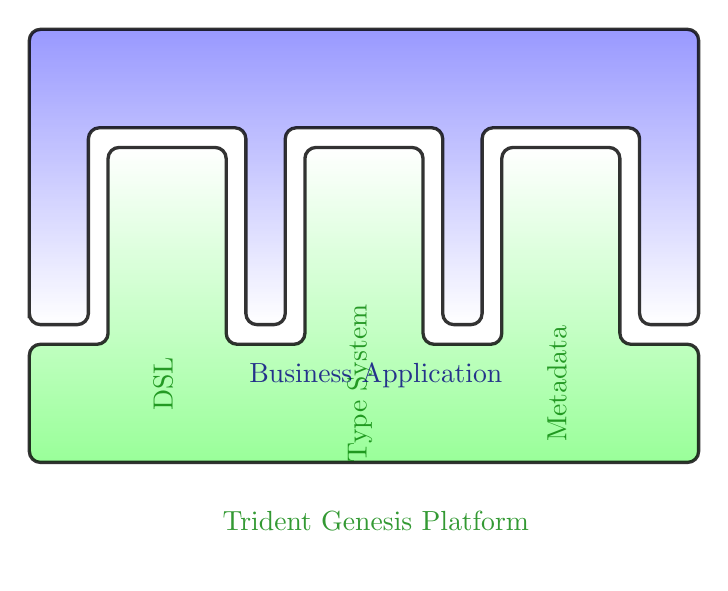
\begin{tikzpicture}[node distance=1cm, auto, opacity=0.8]
      \tikzset{
	  application/.style={rectangle,rounded corners,draw=black, top color=blue!50!white, bottom color=white,very thick, inner sep=1em, minimum size=3em, text centered, text=blue!50!black},
	  platform/.style={rectangle,rounded corners,draw=black, top color=white, bottom color=green!50!white,very thick, inner sep=1em, minimum size=3em, text centered, text=green!50!black},
	  mylabel/.style={text width=7em, text centered} 
      }  
      
      \def\platformpath{-- +(8.5cm,0cm) -- +(8.5cm,1.5cm) -- +(7.5cm,1.5cm) -- +(7.5cm,4.0cm) -- +(6.0cm,4.0cm) -- +(6.0cm,1.5cm) -- +(5.0cm,1.5cm) -- +(5.0cm,4.0cm) -- +(3.5cm,4.0cm) -- +(3.5cm,1.5cm) -- +(2.5cm,1.5cm) -- +(2.5cm,4.0cm) -- +(1.0cm,4.0cm) -- +(1.0cm,1.5cm) -- +(0.0cm,1.5cm) -- cycle}
      
      \draw (-1,-1.5) [platform] \platformpath
	    node [below, text width=3.5cm, text centered, yshift=1.0cm, xshift=1.15cm, rotate=90] {DSL}
	    node [below, text width=3.5cm, text centered, yshift=1.0cm, xshift=3.65cm, rotate=90] {Type System}
	    node [below, text width=3.5cm, text centered, yshift=1.0cm, xshift=6.15cm, rotate=90] {Metadata}
	    node [below, text centered,xshift=4.4cm, yshift=-0.2cm] {Trident Genesis Platform};

      \def\apppath{-- +(0cm,0cm) -- +(0.75cm,0cm) -- +(0.75cm,2.5cm) -- +(2.75cm,2.5cm) -- +(2.75cm,0cm) -- +(3.25cm,0cm) -- +(3.25cm,2.5cm) -- +(5.25cm,2.5cm) -- +(5.25cm,0cm)-- +(5.75cm,0cm)-- +(5.75cm,2.5cm) -- +(7.75cm,2.5cm) -- +(7.75cm,0cm) -- +(8.5cm,0cm) -- +(8.5cm,3.75cm) -- +(0cm,3.75cm) -- cycle}

      \draw (-1,0.25) [application] \apppath node [above, text centered,xshift=4.4cm, yshift=-1.2cm] {Business Application};
    \end{tikzpicture} 
  \end{wrapfigure}
  
  Different general purpose programming languages provide different degrees of support for developing sophisticated internal DSLs.
  For example, scripting languages generally provide better ways of implementing internal DSLs (e.g. Ruby).
  However, in our strong opinion statically typed languages are of essential importance for constructing complex business oriented information systems.
  
  From the very beginning the Trident Genesis Platform was envisaged as an application platform founded on concepts of the internal DSL and domain-driven development (inspired by Eric Evans's ``Domain-Driven Design: Tackling Complexity in the Heart of Software'').
  In order to ensure wider acceptance by the software development community\footnote{Popularisation of the platform among developers and the existence of multiple business applications built on top of it forms a community, which provides an invaluable resource for new developers and helps identifying additional features that should be incorporated into the platform leading to further improvement of its abstraction mechanism.}, the platform taps into the power of modern IDEs and existing programming skills of software developers using the Java programming language\footnote{Java is not the best host language for developing internal DSLs (e.g. Scala is a lot more adequate), but the maturity of the existing Java infrastructure and the development experience played a critical part in this decision.}.
  The internal DSLs are used for expressing the application's behaviour in a declarative way addressing key areas of any software solution such as web, database communication and the user interface design.

\subsection{Type System and Metadata}
  The concept of \emph{metadata driven} software development is well accepted and rapidly gaining its popularity among practitioners, affecting all modern software platforms and frameworks.
  The TG platform provides its unique type system and metadata support specifically targeted at the development of business applications.
  The core of any TG-based applications is formed out of types modeling the business entities and the metadata, which complements the types.
  Together types and metadata define the object hierarchy used for building all main parts of the business application as well as for determining all aspect of its behaviour.
  Basically, the execution of such business applications effectively interprets the developed types and metadata, which provides all necessary application functionality.

  The business domain entities are modeled by reusing provided in the platform type system, which supports well-defined patterns for modeling real-life interoperability between domain entities.  
  Metadata provides a declarative way to associate various business rules with domain entities (e.g. validation rules), define application security, control transaction demarcation, visual representation of domain entities and more.
  It also assists in fine-tuning of the business domain models with the support for configuration-based behaviour achieved by means of dependency injection.
  
  \begin{wrapfigure}{r}{50mm}
    \vspace{-30pt}
    \centering    
    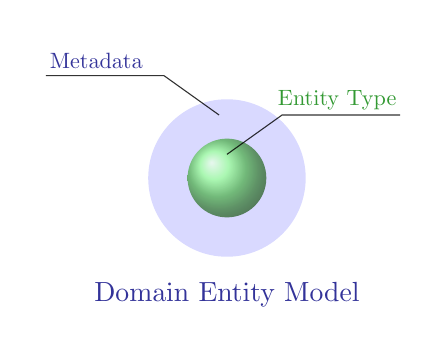
\begin{tikzpicture}[node distance=1cm, auto, opacity=0.8]
      \tikzset{
	  arrow/.style={draw=black, thin, inner sep=1em, minimum size=3em, text centered}
      }      
      \fill[circle, color=blue!50!white, opacity=0.3] (0,0) circle (1.0cm);
      \shade[ball color=green!50!white] (0, 0) circle (0.5cm)  node [below,text=blue!50!black,yshift=-1.2cm] {Domain Entity Model};
      
      \def\corearrow{+(0cm,0cm) -- +(0.7cm,0.5cm) -- +(2.2cm,0.5cm)}

      \draw (0.0,0.3) [arrow] \corearrow node [above,text=green!50!black,scale=0.8,xshift=-1.0cm,yshift=-0.3cm] {Entity Type};
      \draw (0.1,0.8) [arrow, xscale=-1] \corearrow node [above,text=blue!50!black,scale=0.8,xshift=0.8cm,yshift=-0.3cm] {Metadata};
    \end{tikzpicture} 
    \vspace{-30pt}
  \end{wrapfigure}

  By describing the application in terms of types and metadata, the developer informs the platform of a lot of useful information, which can be used by the platform in many different ways.
  Based on this information, the platform automatically constructs a large part of the application internals, which provides the support for a complete application life-cycle.
  For instance, provided metadata and types are sufficient for automatic construction of the application user interface that leverages the declared validation rules and dependencies between domain entities.
  Even more, the platform utilises this information for providing experienced end-users (i.e. without programming skills) of the business application with facilities to build comprehensive reports and analyses.

  So, the basic idea behind the type system and metadata driven approach to model the business domain is to depart from the old imperative paradigm towards the declarative way of defining the information system while remaining in the realm of the pure Java programming language\footnote{TG strives to confine the application development process to the use of Java only without the need for XML or any other external to Java language for modeling the business domain.}.
  
  \subsection{Model Driven Architecture}
  Trident Genesis enforces a strict orientation on model-driven development of business applications.
  The notion of \emph{model} here means not only the business model as outline previously, but the a complete programming model supported by the platform.
  This includes approaches for constructing data structures, implementation of the business logic, the ways of binding domain entities and user interface components, layouting application functionality at different layers and more.

  The major advantage of the enforced model is that all TG-based applications follow exactly the same development model, which ensures structural and behavioural uniformity.
  When the developer needs to implement a specific feature of some particular business domain, the platform provides a well-defined set of approaches for achieving it.
  On the one hand, such strict model enforcement limits the freedom of developers\footnote{This is done purposefully.}, but on the other hand this protects them from multitude of programming errors provisioning for getting a working solution in short terms, which can be easily supported\footnote{Due to the platform uniform programming model.} by the original or new developers.

  One of the obvious results of this is the isolation of software developers working on business solutions from many technical details such as data storage, application layering, handling of web communication etc.
  For example, as has been already mentioned, developers can easily specify a different database engine without any applications modification, or they can adjust descriptions of business entities without the need to update any user interfaces.
  Data manipulation is also performed at the high-level programming model, which is interpreted by the platform in accordance with the specified database engine.
  
  Having a unified well-defined programming model significantly simplifies and improves comprehensibility of TG-based business applications, which further contributes to ease of application development and support.
  Application development is completely done in the same system of concepts, which establishes a ubiquitous language carried out through all stages of development and support for all applications.
  Developers do not need to learn new concepts when supporting different TG-based applications and loose time otherwise required for switching between non-uniformly developed applications\footnote{This platform's singularity provides a way for establishing a Software Product Line for business solutions targeted at a specific problem domain.}.
  
  For example, the business entities modeled with platform's type system and metadata mechanism uniformly determine respective data structures in the underlying database.
  Any manipulation of business entities is done in the same way regardless of whether it is the applications served side or the client side without concerning at what architectural layer these manipulations need to occur.
  Thus, there is no need to switch between SQL when requesting data from a database and some HTTP specific API when communicating with a web resource.

  Our estimations based on the experience building TG-based applications suggests that providing the unified programming model yields an order of magnitude higher performance creating new and modifying existing business applications.

\subsection{Domain Model Reuse}
  One of the questions that is frequently raised when developing business solutions is the ability to reuse certain functionality between two or more applications.
  This is especially critical if there are several business applications developed for the same or similar business domain, but different customers, as it would greatly simplify and improve application support (common enhancements, bug fixes etc.).
  There are two distinct building blocks of any business application, which might need to be reused.
  \begin{itemize}
   \item \emph{Technical infrastructure} -- this is everything that has to do with technical aspects of software development and execution; it is critical to software applications, but brings the business value indirectly by making things possible.
    \item \emph{Business domain model} --  this is the part of business applications, which has a direct correspondence to the actual business practices benefiting from software automation; thus representing the most valuable software asset to the business.
  \end{itemize}

  \begin{wrapfigure}{l}{90mm}
    \vspace{-15pt}
    \centering    
    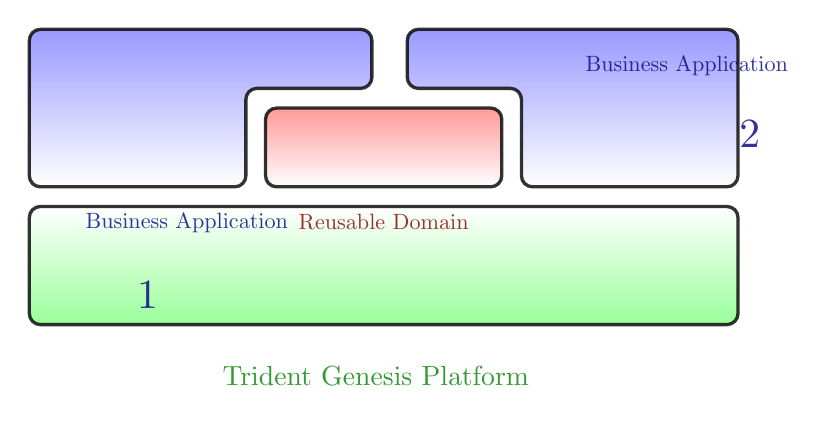
\begin{tikzpicture}[node distance=1cm, auto, opacity=0.8]
      \tikzset{
	  application/.style={rectangle,rounded corners,draw=black, top color=blue!50!white, bottom color=white,very thick, inner sep=1em, minimum size=3em, text centered, text=blue!50!black},
	  reusableblock/.style={rectangle,rounded corners,draw=black, top color=red!50!white, bottom color=white,very thick, inner sep=1em, minimum size=3em, text centered, text=red!50!black},
	  platform/.style={rectangle,rounded corners,draw=black, top color=white, bottom color=green!50!white,very thick, inner sep=1em, minimum size=3em, text centered, text=green!50!black},
	  mylabel/.style={text width=7em, text centered} 
      }  
      
      \def\platformpath{-- +(9cm,0cm) -- +(9cm,1.5cm) -- +(0.0cm,1.5cm) -- cycle}

      \def\reusabledomain{-- +(3cm,0cm) -- +(3cm,1cm) -- +(0.0cm,1cm) -- cycle}

      \def\appathone{-- +(2.75cm,0cm) -- +(2.75cm,1.25cm) -- +(4.35cm,1.25cm) -- +(4.35cm,2cm) -- +(0cm,2cm) -- cycle}
      \def\appathtwo{+(1.6cm,1.25cm) -- +(1.6cm,0cm) -- +(4.35cm,0cm) -- +(4.35cm,2cm) -- +(0.15cm,2cm) -- +(0.15cm,1.25cm) -- cycle}

      \draw (0,0) [platform] \platformpath  node [below, text centered,xshift=4.4cm, yshift=-0.1cm] {Trident Genesis Platform};
      \draw (3,1.75) [reusableblock] \reusabledomain  node [below, text centered,xshift=1.5cm, scale=0.8] {Reusable Domain};
      \draw (0,1.75) [application] \appathone node [above, text centered,xshift=2.0cm, yshift=-0.9cm, scale=0.8] {Business Application} node [above, text centered,xshift=1.5cm, yshift=-2.2cm, scale=1.5] {1};
      \draw (4.65,1.75) [application] \appathtwo node [above, text centered,xshift=2.1cm, yshift=-0.15cm, scale=0.8] {Business Application } node [above, text centered,xshift=2.9cm, yshift=-1.4cm, scale=1.5] {2};
    \end{tikzpicture} 
    \vspace{-30pt}
  \end{wrapfigure}

  The Trident Genesis platform incorporates the \emph{technical infrastructure} reused by all TG-based business applications.
  This completely eliminates any work on part of application developers otherwise required to ensure reuse of this building block across multiple applications.
  The platform takes care of updates such as improvements to the underlying algorithms, handles API enhancements, backward compatibility and more.
  Of course, there is no such thing as a free lunch -- all the complexity of supporting the technical infrastructure that enables natural reuse by all TG-based business solutions is hidden into the platform itself, shifting full responsibility to the platform developers\footnote{This is only natural and ensures clear responsibility separation. Such practices correspond to world-class software developments such as the Oracle Java Virtual Machine. 
  Applications written for JVM are not concerned with the reuse of JMV as it occurs intrinsically. Similarly happens with TG-based applications, but at the higher level of abstraction.}.

  \emph{Business domain models} (or simply \emph{domain models}) belong to the realm of the business application development.
  The provided by the platform development model is well-suited for building reusable domain models.
  Due to its highly modular nature, the platform greatly facilitates modularity at the application level.
  There is a clear cut between all the constructs used for implementing domain models, which are woven together by means of injection of control.
  This, for example, allows sharing the same domain entities without any modification as a separate module with capability to provide different business rules for their validation, which could be customer specific.

  Thus, the Trident Genesis platform has an intrinsic nature for sharing technical infrastructure and provides rich functionality for reuse of business domain models and logic between multiple business applications.